% !TeX spellcheck = en_US
\section{Freedom of information and public access}
\subsection{Separation of powers}
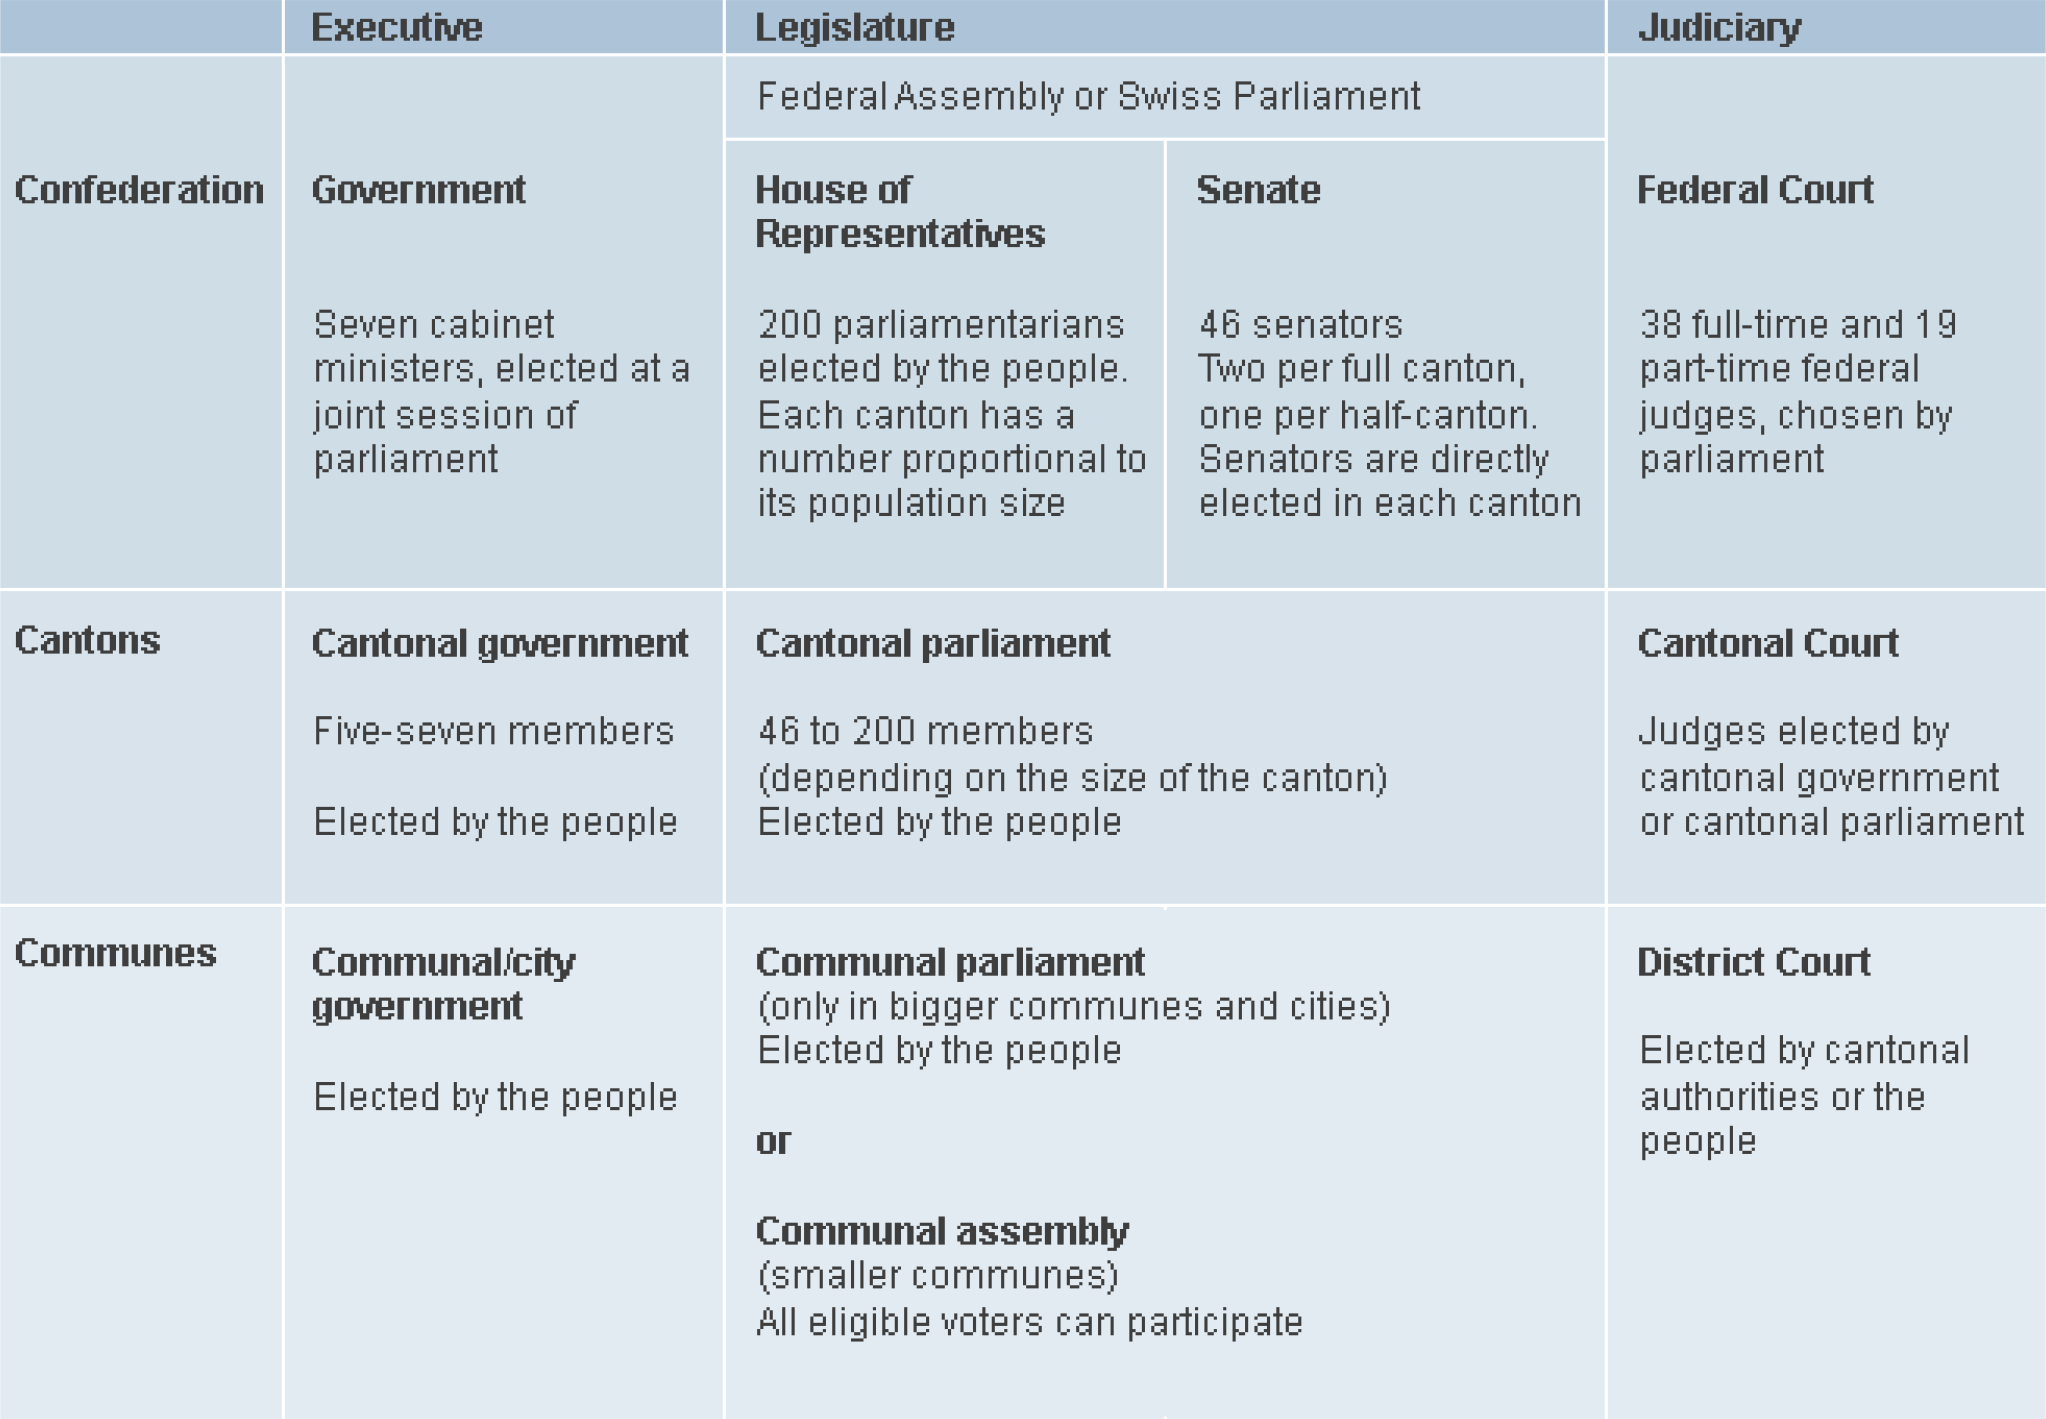
\includegraphics[width=1\linewidth]{images/separation_of_powers}

\subsection{Direct democracy}
\begin{compactitem}
	\item Direct democracy means the citizens are the sovereign and decide policy, i.e. legislation directly, by votes on initiatives and referendums on changes to the constitution or enactment of a law. The majority of modern democracies are “only” representative democracies in which people vote for representatives who then enact policy initiatives.
	\item Switzerland is a rare example of a country with instruments of direct	democracy at the levels of the municipalities, cantons, and federal state. Citizens have more power than in a representative democracy. No other country gives its citizens more opportunities to express their views in popular votes on more issues than in Switzerland. The People are sovereign, the highest political authority in the land. All Swiss citizens with full legal capacity – over 5.2 million men and women - have the right to vote.
	\item On any political level citizens can propose changes to the constitution (popular initiative), or ask for a optional referendum to be held on any law voted by the federal, cantonal parliament and/or municipal legislative body.
\end{compactitem}

\subsection{What are the aims of Freedom of Information?}
Access of the general public to information of the government is considered	of fundamental importance for the effective functioning of democratic systems:
\begin{compactenum}
	\item Element of the fundamental right of freedom of expression set forth by Article 19 of the Universal Declaration of Human Rights (1948).
	\item It enhances governments and public officials accountability, trustworthiness and credibility (Checks and Balances!)
	\item It enhances people participation by allowing their informed participation.
	\item Democracy can only thrive if the media as the “fourth power” has access to information of the government.
\end{compactenum}

\subsection{Freedom of Information in the World}
\begin{compactitem}
	\item Over the past 10 years, the right to information and access to public information has been recognised in an increasing number of countries.
	\item Several laws have been adopted all over the world, including in the developing countries. In 1990 only 13 countries had a national freedom of	information law, today there are 100 such laws across the world.
	\item The Fall of the Berlin Wall and the rapid growth of civil society groups demanding access to information gave impetus to the next wave of	enactments.
	\item As of May 2012, when Brazil's law entered into force, more than 5.5 billion people live in countries that include in their domestic law an enforceable right, at least in theory, to obtain information from their governments.
\end{compactitem}

\subsection{Freedom of Information in Switzerland}
Freedom of expression, a fundamental right of the constitution, includes the right to receive, access and share information without being restricted by authorities.\\
Like every fundamental right, the freedom of expression is not absolute and may be limited if there are overriding public or private interests.

\subsection{Freedom of Information on Federal Level}
The Federal Act on Freedom of Information in the Administration entered into force on 1 July 2006.\\
It introduced a paradigm shift from the non-disclosure principle to the transparency principle by granting greater freedom of information.\\
The Freedom of Information Act only applies to
\begin{compactitem}
	\item official documents created by the Federal Government, ie. Federal Administration, Parliamentary Services, and public and private persons and organisations when acting in official capacity and issuing decrees or rulings (eg. POST, SBB)
	\item Official documents are all those containing information concerning public duties
	\item official documents created after 1 July 2006.
\end{compactitem}
\textbf{Exceptions:}\\
Not subject to access by the public are for example:
\begin{compactitem}
	\item Documents of the Parliament
	\item Information used commercially by an authority (e.g. maps from the Federal	Office of Topography)
	\item Official documents which have not yet been completed .
	\item Documents intended for personal use by government officials (eg. handwritten notes, working copies of documents or personal memos)
\end{compactitem}
\textbf{Application for access:}
\begin{compactitem}
	\item Anybody is entitled to apply to access documents!
	\begin{compactitem}
		\item Irrespective of where they live or of their nationality.
		\item Even legal entities and associations
	\end{compactitem}
	\item No particular form for the application
	\begin{compactitem}
		\item In writing, via e-mail
		\item orally (eg. by phone or in person) or in written form, by letter, fax or e-mail.
		\item No reason must be given for applying and the applicant does not have to declare any particular interest or personal motive or even a personal involvement.
	\end{compactitem}
\end{compactitem}
\textbf{Content of Application for Access:}\\
The application must be sufficiently precise! It must contain enough detail to allow identification of the required
documents:
\begin{compactitem}
	\item date or period of creation
	\item title or reference, exact subject matter,
	\item the authority which may have published documents on the subject
\end{compactitem}
Where required, the authority may ask the applicant to give more precise information. The authority must support the applicant in its application, meaning it cannot immediately reject the application if it is not precise enough.\\
\textbf{Fees for Access:}\\
Access to official documents is normally subject to a fee. Fees are regulated by ordinance: 100 CHF per hour.
\begin{compactenum}
	\item The authority must inform the applicant in advance of the amount of fees.
	\item The applicant can decide on whether to continue with the application within 10 days.
	\item If no decision by the applicant is submitted within 10 days, the application is deemed withdrawn.
	\item The authority may reduce the fees if it decides to reject the application or only permit partial access.
\end{compactenum}
\textbf{Process for Access:}\\
The authority should respond to the application within 20 days. This deadline may be extended under only if:
\begin{compactitem}
	\item The official documents are too long, complex or difficult to obtain,
	\item The official documents contain personal data
\end{compactitem}
The authority must inform the applicant if the processing deadline is extended. If the authority does not respond to an application within the prescribed period, the applicant can submit a written request for mediation to the Federal Data Protection and Information Commissioner within 20 days.\\
\textbf{Restrictions of Access in the Public Interest:}
\begin{compactitem}
	\item The right of access may be limited or refused if the document may compromise an overriding public interest.
	\item The Freedom of Information Act contains several exceptions relating to special cases in which access can be limited, deferred or refused. For example if allowing access to official documents would mean that
	\begin{compactitem}
		\item Switzerland's internal or external security could be jeopardized;
		\item Switzerland's foreign policy interests or international relations could be compromised;
		\item relations between the Confederation and Cantons or between Cantons could be compromised;
		\item Switzerland's economic, financial or monetary policy interests could be jeopardized.
	\end{compactitem}
	\item If access is limited or refused, the authority must justify its decision.
	\item The applicant can submit a written request for mediation to the Federal Data Protection and Information Commissioner within 20 days.
\end{compactitem}
\textbf{Restrictions of Access to protect a Private Interest:}
\begin{compactitem}
	\item The right of access may be limited if the document may compromise an overriding private interest.
	\item The Furthermore, it may be necessary to limit, defer or refuse access in order to protect
	\begin{compactitem}
		\item Personal data of third parties;
		\item Confidential information of third parties
		\item Intellectual property of third parties
		\item Professional, business and industrial secrets of third parties.
	\end{compactitem}
	\item If access is limited or refused, the authority must justify its decision.
	\item The applicant can submit a written request for mediation to the Federal Data Protection and Information Commissioner within 20 days.
\end{compactitem}

\subsection{Role of the Federal Data Protection and	Information Commissioner}
Federal Data Protection and Information Commissioner has been assigned a number of functions:
\begin{compactitem}
	\item He informs and advises private citizens on how to gain access to official documents.
	\item He advises the various administrative authorities and federal departments on the implementation of the Federal Act on Freedom of Information in the Administration.
	\item He acts as mediator in the event of a disagreement.
	\item He gives an opinion on draft legal texts prepared by the federal authorities that have an impact on the principle of transparency.
\end{compactitem}
Federal Data Protection and Information Commissioner is independent!

\subsection{Legal base}
\subsubsection{Freedom of expression and of information - ART. 16 Federal Constitution}
\begin{compactenum}
	\item Freedom of expression and of information is guaranteed.
	\item Every person has the right freely to form, express, and impart their opinions.
	\item Every person has the right freely to receive information to gather it from generally accessible sources and to disseminate it.
\end{compactenum}	

\textit{\begin{compactenum}
	\item Die Meinungs- und Informationsfreiheit ist gewährleistet.
	\item Jede Person hat das Recht, ihre Meinung frei zu bilden und sie ungehindert zu äussern und zu verbreiten.
	\item Jede Person hat das Recht, Informationen frei zu empfangen, aus allgemein zugänglichen Quellen zu beschaffen und zu verbreiten.
\end{compactenum}}

\subsubsection{Freedom of the media - ART. 17 Federal Constitution}
\begin{compactenum}
	\item Freedom of the press, radio and television and of other forms of dissemination of features and information by means of public telecommunications is guaranteed.
	\item Censorship is prohibited.
	\item The protection of sources is guaranteed.
\end{compactenum}

\textit{\begin{compactenum}
	\item Die Freiheit von Presse, Radio und Fernsehen sowie anderer Formen der öffentlichen fernmeldetechnischen Verbreitung von Darbietungen und Informationen ist gewährleistet.
	\item Zensur ist verboten.
	\item Das Redaktionsgeheimnis ist gewährleistet.
\end{compactenum}}
